% ---- figure comparaison_distances_line_graphes_cellules_k_2x50
\begin{figure}[htb!] 
\centering
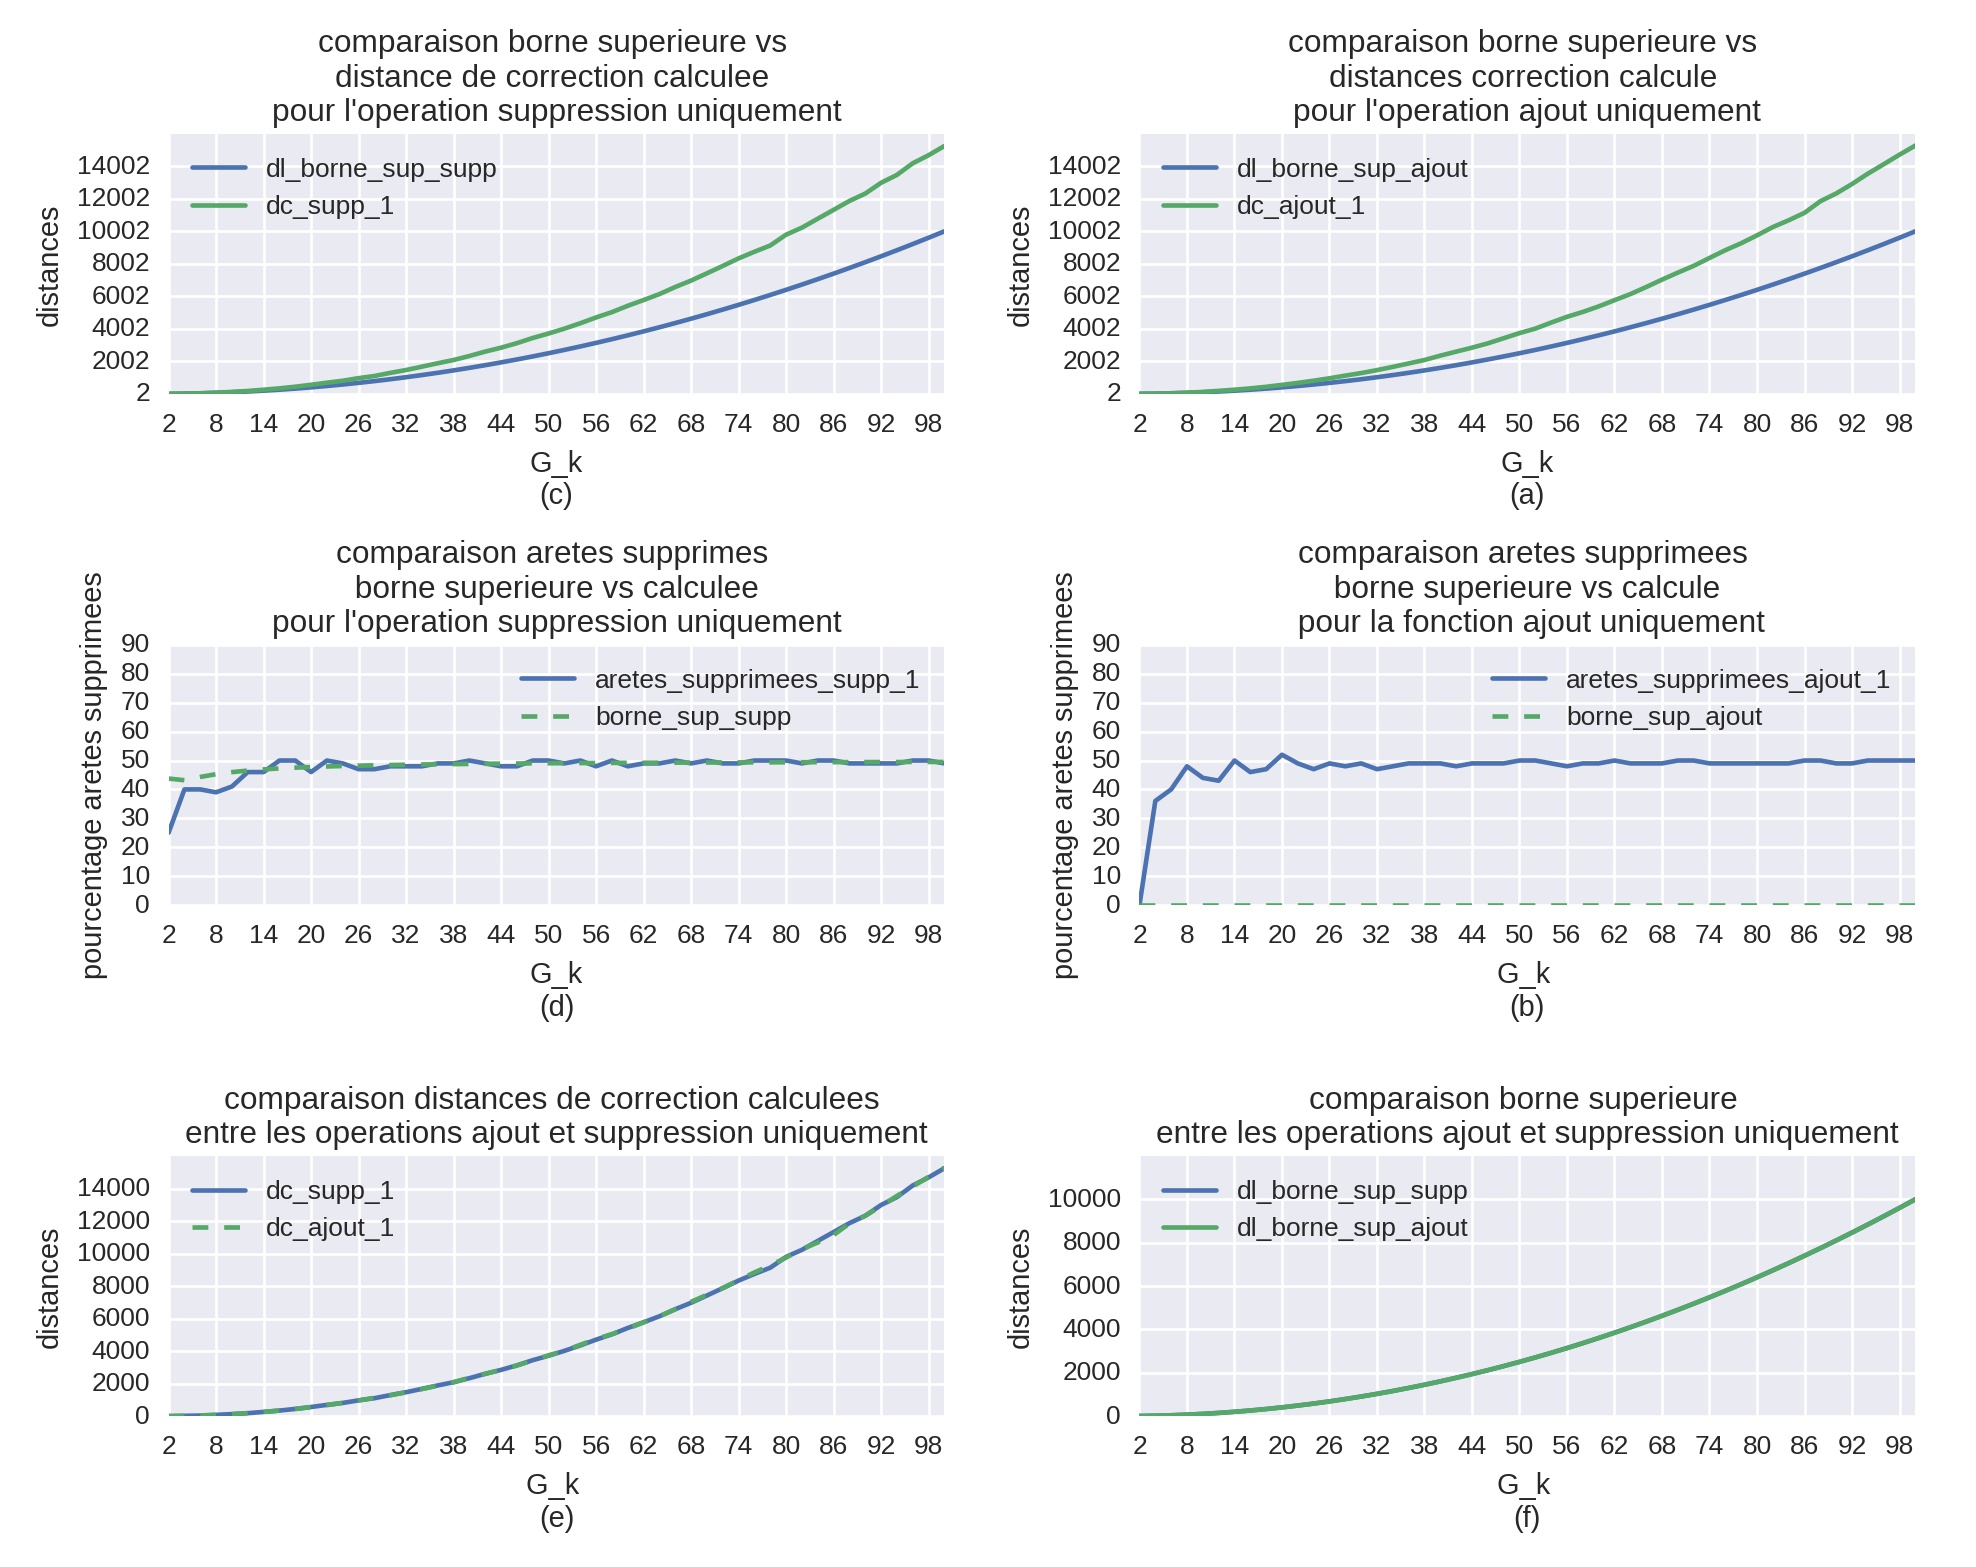
\includegraphics[scale = 0.25]{comparaison_distances_line_graphes_cellules_k_2x50.jpeg}
\caption{Comparaison des distances lines th\'eoriques et calcul\'ees selon des fonctions de co\^ut {\em suppression} et  {\em ajout}.
La figure $(a)$ d\'esigne la comparaison de distances line pour la fonction {\em ajout} entre les distances th\'eoriques et celles obtenues apr\`es l'ex\'ecution de l'algorithme de correction. 
La figure $(b)$ repr\'esente la comparaison entre les ar\^etes supprim\'ees th\'eoriques et celles obtenues apr\`es la correction pour la fonction {\em ajout}.
La figure $(c)$ repr\'esente la comparaison entre les distances line th\'eoriques et celles obtenues apr\`es la correction pour la fonction {\em ajout}.
La figure $(d)$ repr\'esente la comparaison entre les ar\^etes supprim\'ees th\'eoriques et celles obtenues apr\`es la correction pour la fonction {\em suppression}.
La figure $(e)$ repr\'esente la comparaison des distances line obtenues apr\`es l'ex\'ecution de l'algorithme de correction entre les fonctions {\em suppression} et {\em ajout}.
La figure $(f)$ repr\'esente la comparaison des distances line th\'eoriques entre les fonctions {\em suppression} et {\em ajout}.
}
\label{comparaison_distances_line_graphes_cellules_k_2x50}
\end{figure}
% ---- figure comparaison_distances_line_graphes_cellules_k_2x50

Nous r\'ealisons cinq comparaisons et les r\'esultats obtenus sont regroup\'es en $6$ exp\'erimentations.
\newline
Les deux premi\`eres exp\'erimentations comparent les distances line th\'eoriques et celle obtenues apr\`es l'ex\'ecution de nos algorithmes pour chaque fonction de co\^ut. Le terme {\em th\'eorique} signifie que le line-graphe obtenu apr\'es la correction du graphe cellule $G_k$ est optimal c'est-\`a-dire la distance line de $G_k$ est minimale. 
La figure \ref{comparaison_distances_line_graphes_cellules_k_2x50}(c) d\'esigne la comparaison avec la fonction {\em suppression} entre la distance line th\'eorique {\em dl\_theorique\_supp} et la distance line calcul\'ee {\em dl\_supp\_1}. Alors que la fonction {\em ajout} est repr\'esent\'ee par la figure \ref{comparaison_distances_line_graphes_cellules_k_2x50}(a) dans laquelle nous comparons les distances line th\'eoriques {\em dl\_theorique\_ajout}  et calcul\'ees {\em dl\_ajout\_1}.  

Les  exp\'erimentations  des figures \ref{comparaison_distances_line_graphes_cellules_k_2x50}$(d)$ et \ref{comparaison_distances_line_graphes_cellules_k_2x50}$(b)$ indiquent, respectivement, le pourcentage d'ar\^etes supprim\'ees dans les graphes $G_k$ pour les fonctions de co\^ut {\em suppression} et {\em ajout}. Nous avons determin\'e th\'eoriquement le nombre d'ar\^etes \`a supprimer pour obtenir le line-graphe optimal et nous comparons ce nombre avec celui des ar\^etes supprim\'ees apr\'es l'ex\'ecution des algorithmes. 
Les termes {\em aretes\_G\_k\_notIn\_LG\_theoriques\_supp} et {\em aretes\_G\_k\_notIn\_LG\_theoriques\_ajout} d\'esignent, respectivement, la courbe th\'eorique des ar\^etes supprim\'ees dans les graphes $G_k$ pour fournir des line-graphes optimaux avec la fonction {\em suppression} et {\em ajout}. De m\^eme, les termes {\em aretes\_G\_k\_notIn\_LG\_supp\_1} et  {\em aretes\_G\_k\_notIn\_LG\_ajout\_1} d\'esignent, respectivement, la courbe des ar\^etes supprim\'ees dans les graphes $G_k$ apr\`es l'ex\'ecution des algorithmes pour les fonctions {\em suppression} et {\em ajout}.

La figure \ref{comparaison_distances_line_graphes_cellules_k_2x50}$(e)$ repr\'esente la comparaison entre les distances line qui sont calcul\'ees avec les diff\'erentes fonctions de co\^ut. Ainsi, {\em dl\_ajout\_1} et {\em dl\_supp\_1} identifient, respectivement, les courbes avec les fonctions {\em ajout} et {\em suppression}. 
De m\^eme, la figure \ref{comparaison_distances_line_graphes_cellules_k_2x50}$(f)$ compare les distances line th\'eoriques avec les diff\'erentes fonctions de co\^ut. Ainsi, {\em dl\_theorique\_supp} et {\em dl\_theorique\_ajout} identifient, respectivement, les courbes avec les fonctions {\em suppression} et {\em ajout}. 
\newline

Dans les figures $(a)$ et $(c)$ , nous constatons que les distances line th\'eoriques sont inf\'erieures aux distances line obtenues apr\`es l'algorithme de correction, peu importe la fonction de co\^ut.
L'\'ecart du nombre d'ar\^etes entre les distances lines th\'eoriques {\em dl\_theorique\_ajout} et celle calcul\'ees {\em dl\_ajout} dans la fonction {\em ajout} provient des ar\^etes ajout\'ees entre deux cellules partageant un sommet. Ces ar\^etes sont ajout\'ees entre un sommet de chaque cellule et cela entraine la suppression d'ar\^etes de $G_k$  car la suppression d'ar\^etes lors d'un partitionnement en cliques se r\'ealise sur les aretes de $G_k$. Aussi ces ar\^etes ajout\'ees provoquent l'abandon d'ar\^etes diagonales ajout\'ees \`a partir du sommet commun dans les cellules comme indiqu\'e dans l'exemple du graphe $G_{3,3}$ dans la figure \ref{exempleCorrectionGrapheCelluleAvecAjout}. 
Les ar\^etes supprim\'ees avoisinent en moyenne $40\%$ quand le nombre de cellules est faible $k\le13$. Au d\'el\`a de $k > 13$, une ar\^ete sur deux du graphe $G_{k}$ est supprim\'ee comme il est indique dans la figure $(b)$.
La courbe de {\em aretes\_G\_k\_notIn\_LG\_ajout\_1} est nulle parce que nous ne supprimons aucune ar\^ete dans le line-graphe $L(G_k)$ optimal.
Quant aux cellules ayant une ar\^ete commune, une seule ar\^ete diagonale est ajout\'ee dans chaque cellule \`a partir du m\^eme sommet de l'ar\^ete commune.  
\newline  
En ce qui concerne  l'\'ecart entre le nombre d'ar\^etes supprim\'ees th\'eoriques et calcul\'ees, nous pouvons dire que les ar\^etes issues de cet \'ecart proviennent de cellules voisines. Dans les cellules partageant un sommet, l'algorithme ajoute g\'en\'eralement une ar\^ete diagonale \`a partir de ce sommet commun dans une seule cellule. Les ar\^etes diagonales ajout\'es sont responsables de l'augmentation de la distance line {\em dl\_supp\_1}.
Pour des cellules partageant une ar\^ete, l'algorithme supprime l'ar\^ete commune.  Cela explique pourquoi nous avons en moyenne $50\%$ des ar\^etes de $G_k$ qui sont supprim\'ees dans la figure $(d)$ et ce pourcentage est identique avec les ar\^etes supprim\'ees th\'eoriques lorsque le nombre de cellules devient \'elev\'e $k \ge 17$.
\newline
Par ailleurs, 
nous avons en moyenne $2/3$ ar\^etes ajout\'ees et $1/3$ d'ar\^etes supprim\'ees dans les distances line {\em dl\_ajout\_1}. Et dans les distances {\em dl\_supp\_1}, $2/3$ ar\^etes sont des ar\^etes supprim\'ees et $1/3$ sont des ar\^etes ajout\'ees.
Ceci implique que les courbes des distances   {\em dl\_ajout\_1} et {\em dl\_supp\_1} ont les m\^emes tendances et sont superpos\'ees (figure $(e)$). 
La superposition des distances line th\'eoriques des diff\'erentes fonctions (figure $(f)$) est due \`a l'ordre de l'expression litt\'erale de leurs distances. En effet, le d\^egre de polyn\^omes des fonctions {\em ajout} et {\em suppression} est $2$ et les coefficents de ces polyn\^omes sont tr\`es proches.
\newline

L'exp\'erimentation montre que les line-graphes $L(G_k)$ propos\'es par l'algorithme de correction sont identiques  en terme de distance line quelle que soit la fonction de co\^ut. Toutefois, les solutions propos\'ees ne sont pas optimales parce que l'algorithme supprime des ar\^etes pendant la fonction {\em ajout} et ajoute des ar\^etes pendant la fonction {\em suppr\'ession}.  
